\documentclass{article}%
\usepackage[T1]{fontenc}%
\usepackage[utf8]{inputenc}%
\usepackage{lmodern}%
\usepackage{textcomp}%
\usepackage{lastpage}%
\usepackage[head=40pt,margin=0.5in,bottom=0.6in]{geometry}%
\usepackage{graphicx}%
%
\title{\textbf{Delegado de Acnur y OIM para el éxodo venezolano llega mañana a Colombia}}%
\author{EFE}%
\date{14/10/2018}%
%
\begin{document}%
\normalsize%
\maketitle%
\textbf{URL: }%
http://www.eluniversal.com/politica/23173/delegado{-}de{-}acnur{-}y{-}oim{-}para{-}el{-}exodo{-}venezolano{-}llega{-}manana{-}a{-}colombia\newline%
%
\textbf{Periodico: }%
EU, %
ID: %
23173, %
Seccion: %
politica\newline%
%
\textbf{Palabras Claves: }%
NO\_TIENE\newline%
%
\textbf{Derecho: }%
CONTEXTO, %
Otros Derechos: %
18, %
Sub Derechos: %
\newline%
%
\textbf{EP: }%
NO\newline%
\newline%
%
\textbf{\textit{El representante de la Acnur y la OIM, Eduardi Stein, será recibido por el canciller Carlos Holmes Trujillo, junto a quien dará una rueda de prensa para comentar sus expectativas acerca de la visita}}%
\newline%
\newline%
%
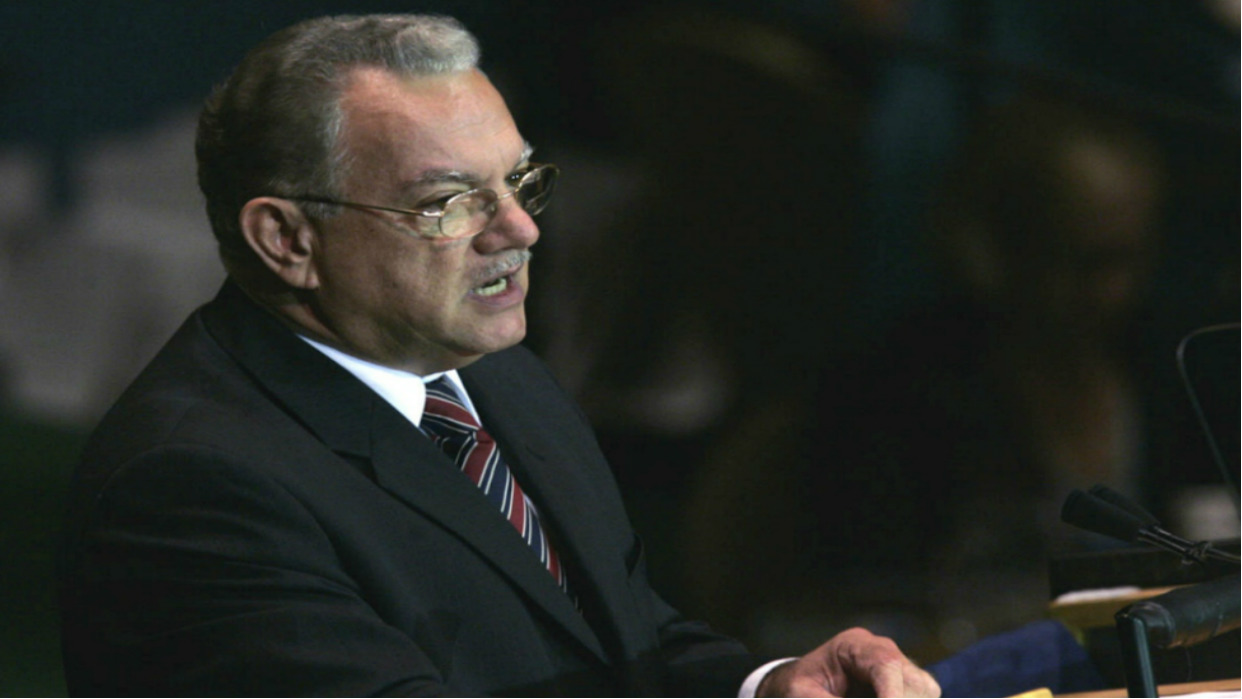
\includegraphics[width=300px]{76.jpg}%
\newline%
%
Bogotá.{-}El representante de la Agencia de la ONU para los Refugiados (Acnur) y de la Organización Internacional para las Migraciones (OIM) para los refugiados y migrantes venezolanos, Eduardo Stein, iniciará mañana una visita a Colombia para conocer de primera mano la situación.%
\newline%
%
A su llegada al aeropuerto El Dorado de Bogotá será recibido por el canciller Carlos Holmes Trujillo, junto a quien dará una rueda de prensa para comentar sus expectativas acerca de la visita.%
\newline%
%
Precisamente desde que asumió su cargo como ministro de Relaciones Exteriores, Trujillo ha trabajado para hacer visible el impacto regional por la crisis causada por el éxodo de cerca de 2,3 millones de venezolanos que han abandonado su país, Efe.%
\newline%
%
De ellos, casi un millón se han asentado en Colombia, un país al que cruzan cerca de 35.000 venezolanos diariamente, algunos en busca de comida y medicamentos, otros para dejar atrás definitivamente la crisis.%
\newline%
%
El Gobierno colombiano estima que el número de venezolanos que lleguen al país puede elevarse hasta los cuatro millones en el escenario más pesimista de un agravamiento de la crisis.%
\newline%
%
Stein, que fue vicepresidente de Guatemala entre 2004 y 2008, se reunirá con el jefe de Estado de Colombia, Iván Duque, el martes, así como con Trujillo.%
\newline%
%
Duque explicó ayer que pedirá a su homólogo francés, Emmanuel Macron, el papa Francisco y las autoridades de la Unión Europea (UE) que se agilicen los mecanismos de ayuda ante la crisis migratoria.%
\newline%
%
Duque hará una visita a Europa la próxima semana en la que tiene previsto reunirse con Francisco el 22 de octubre, el 24 de octubre visitará la sede de la Unión Europea (UE) en Bruselas y se encontrará con Macron en una fecha que todavía no se ha hecho pública.%
\newline%
%
\end{document}